\documentclass{article}
\newif\ifshowsolutions
\showsolutionstrue
\usepackage{listings}
\usepackage{amsmath}
%\usepackage{subfigure}
\usepackage{subfig}
\usepackage{amsthm}
\usepackage{amsmath}
\usepackage{amssymb}
\usepackage{graphicx}
\usepackage{mdwlist}
\usepackage{array}
\usepackage{booktabs}
\usepackage{tabularx}
\usepackage[colorlinks=true]{hyperref}
\usepackage{geometry}
\usepackage{titlesec}
\geometry{margin=1in}
\geometry{headheight=2in}
\geometry{top=2in}
\usepackage{palatino}
\usepackage{mathrsfs}
\usepackage{fancyhdr}
\usepackage{paralist}
\usepackage{todonotes}
\setlength{\marginparwidth}{2.15cm}
\usepackage{tikz}
\usetikzlibrary{positioning,shapes,backgrounds}
\usepackage{float} % Place figures where you ACTUALLY want it
\usepackage{comment} % a hack to toggle sections
\usepackage{ifthen}
\usepackage{mdframed}
\usepackage{verbatim}
\usepackage[strings]{underscore}
\usepackage{listings}
\usepackage{bbm}
\rhead{}
\lhead{}

\renewcommand{\baselinestretch}{1.15}

% Shortcuts for commonly used operators
\newcommand{\E}{\mathbb{E}}
\newcommand{\Var}{\operatorname{Var}}
\newcommand{\Cov}{\operatorname{Cov}}
\newcommand{\Bias}{\operatorname{Bias}}
\DeclareMathOperator{\argmin}{arg\,min}
\DeclareMathOperator{\argmax}{arg\,max}

% do not number subsection and below
\setcounter{secnumdepth}{1}

% custom format subsection
\titleformat*{\subsection}{\large\bfseries}

% set up the \question shortcut
\newcounter{question}[section]
\newenvironment{question}[1][]
{\refstepcounter{question}\par\addvspace{1em}\textbf{Question~\Alph{question}\!
\ifthenelse{\equal{#1}{}}{}{ [#1 points]}: }}
{\par\vspace{\baselineskip}}

\newcounter{subquestion}[question]
\newenvironment{subquestion}[1][]
{\refstepcounter{subquestion}\par\medskip\textbf{\roman{subquestion}.\!
\ifthenelse{\equal{#1}{}}{}{ [#1 points]:}} }
{\par\addvspace{\baselineskip}}

\titlespacing
\section{0pt}{12pt plus 2pt minus 2pt}{0pt plus 2pt minus 2pt}
\titlespacing
\subsection{0pt}{12pt plus 4pt minus 2pt}{0pt plus 2pt minus 2pt}
\titlespacing
\subsubsection{0pt}{12pt plus 4pt minus 2pt}{0pt plus 2pt minus 2pt}

\newenvironment{hint}[1][]
{
\begin{em}\textbf{Hint: }}{
\end{em}}

\ifshowsolutions
\newenvironment{solution}[1][]
{\par\medskip
  \begin{mdframed}\textbf{Solution~\Alph{question}#1:}
  \begin{em}}
    {
    \end{em}\medskip
\end{mdframed}\medskip}
\newenvironment{subsolution}[1][]
{\par\medskip
  \begin{mdframed}\textbf{Solution~\Alph{question}#1.\roman{subquestion}:}
  \begin{em}}
    {
    \end{em}\medskip
\end{mdframed}\medskip}
\else
\excludecomment{solution}
\excludecomment{subsolution}
\fi

%%%%%%%%%%%%%%%%%%%%%%%%%%%%%%
% HEADER
%%%%%%%%%%%%%%%%%%%%%%%%%%%%%%

\chead{
  {\vbox{
      Machine Learning \& Data Mining \hfill
      Caltech CS/CNS/EE 155 \hfill \\[1pt]
      Miniproject 1\hfill
      October/November 2026 \\
    }
  }
}

\begin{document}
\pagestyle{fancy}

%%%%%%%%%%%%%%%%%%%%%%%%%%%%%%
% PROBLEM 1
%%%%%%%%%%%%%%%%%%%%%%%%%%%%%%

\newpage

\section{Introduction [15 points]}
\begin{itemize}
  \item Group members: Baaqer Farhat and Andrey Korolev
  \item Kaggle team name: Hood Research Department
  \item Ranking on the private leaderboard: 18 (top 50\%)
  \item AUC score on the private leaderboard: 0.84087
  \item Colab link: \texttt{TBD}
  \item Piazza link: \texttt{TBD}
  \item Division of labor: We divided the work equally between both group
  members. We collaborated on developing and evaluating multiple models,
  tuning their hyperparameters, and combining the strongest models into a
  final ensemble that produced our best predictions.
\end{itemize}
\newpage

\section{Overview [15 points]}
% 1 page maximum
\subsection{Models and techniques attempted}
We started with L2-regularized logistic regression as a simple baseline. We
then trained CatBoost, LightGBM, and XGBoost models because boosted trees can
capture nonlinear relationships between the audio features. We also tested
Random Forest, Extra Trees, Histogram Gradient Boosting, and an Explainable
Boosting Machine. The weaker models were not included in the final prediction.

We tested probability blending, cross-fitted ensemble weights, repeated
fold-and-seed bagging, and rank averaging. We also modified the data by adding
release-date features, audio-feature interactions, track frequency (URI count),
and album-level features. One less standard feature used the nearest tracks
with the same release date in normalized audio-feature space. This was a
fold-safe k-nearest-neighbor feature, not a separate KNN classifier; its
construction is detailed in Appendix Section~\ref{app:knn}. Our final
ensemble rank-averaged predictions from selected LightGBM, XGBoost, CatBoost,
and Extra Trees configurations trained across multiple grouped folds and random seeds. We
also tested release-period specialist models, but only retained changes that
improved grouped validation. Appendix Section~\ref{app:models} explains the
role of each retained model.

\subsection{Work timeline}
\begin{itemize}
  \item \textbf{Monday:} Read the project requirements, inspected the data,
  selected the AUC metric, and planned grouped validation by track URI.
  \item \textbf{Tuesday:} Built the logistic-regression baseline and its
  preprocessing pipeline.
  \item \textbf{Wednesday:} Trained and tuned CatBoost, then reviewed fold
  scores and feature importance.
  \item \textbf{Thursday:} Trained and tuned LightGBM and XGBoost and compared
  their out-of-fold predictions.
  \item \textbf{Friday:} Tested Random Forest, Extra Trees, Histogram Gradient
  Boosting, EBM, and several weighted ensembles.
  \item \textbf{Saturday:} Added release-date, URI-count, album-level,
  interaction, and same-date nearest-neighbor features. We repeated grouped
  cross-validation over several seeds and began testing submissions on Kaggle.
  \item \textbf{Sunday:} Built the final four-model rank-average ensemble,
  tested release-period specialists, continued testing submissions, selected
  our final prediction, and produced report figures and result tables.
\end{itemize}

\newpage

\section{Approach [20 points]}
% 1 page maximum
\subsection{Data exploration, processing and manipulation}
We inspected missing values, class balance, repeated URIs, date formats, and
each feature's relation to popularity.

\noindent
\begin{minipage}[t]{0.43\textwidth}
\vspace{0pt}
\scriptsize
\setlength{\tabcolsep}{3pt}
\renewcommand{\arraystretch}{1.04}
\begin{tabularx}{\linewidth}{@{}>{\raggedright\arraybackslash}p{0.25\linewidth}
  >{\raggedright\arraybackslash}X@{}}
\toprule
\textbf{Group} & \textbf{Processing and purpose} \\
\midrule
Cleaning & Mapped High/Low to 1/0; removed missing URIs, links, and the
constant type field. \\
Logistic & Filled missing values with column medians, scaled audio features,
and encoded categories. \\
Tree models & Kept original numeric scales and used native categories when
supported. \\
Date/audio & Added date components, age, log transforms, and interactions to
expose timing and nonlinear effects. \\
Track/album & Added URI count, date-group size, fold-safe date target means,
and same-date neighbor scores. \\
\bottomrule
\end{tabularx}
\end{minipage}\hfill
\begin{minipage}[t]{0.55\textwidth}
\vspace{0pt}
\centering
\captionsetup{font=footnotesize,skip=2pt}
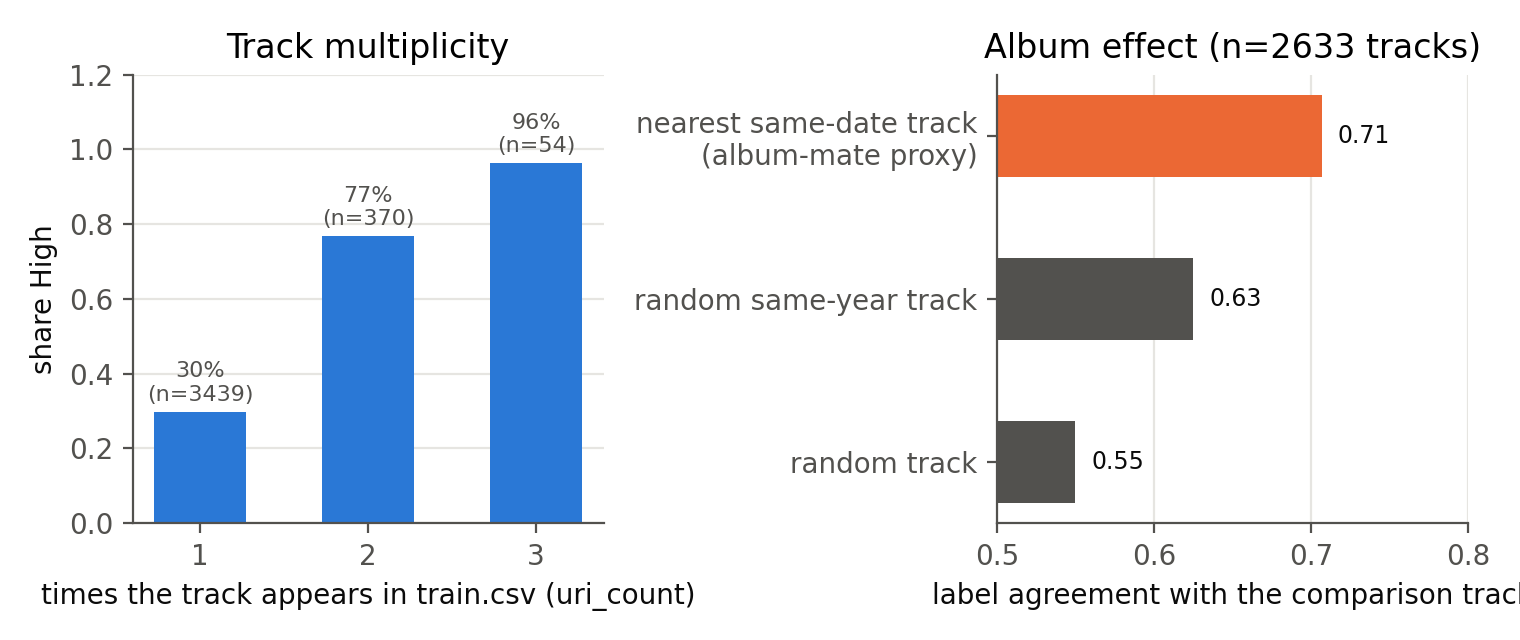
\includegraphics[width=\linewidth]{../final_pipeline/figures/fig_multiplicity_album.png}
\captionof{figure}{Repeated tracks and same-date neighbors contain strong
popularity signals.}
\label{fig:multiplicity-album}
\end{minipage}

Scikit-learn handled missing values, scaling, encoding, and grouped splits.
Label-based album features were rebuilt inside every training fold using inner
URI-grouped folds to prevent leakage. Near-duplicate indicators were tested
but removed because they did not improve validation. Appendix
Section~\ref{app:features} lists the complete feature construction.

\subsection{Details of models and techniques}
\begin{center}
\footnotesize
\setlength{\tabcolsep}{5pt}
\renewcommand{\arraystretch}{1.02}
\begin{tabularx}{\textwidth}{@{}>{\raggedright\arraybackslash}p{0.20\textwidth}
  >{\raggedright\arraybackslash}p{0.31\textwidth}
  >{\raggedright\arraybackslash}X@{}}
\toprule
\textbf{Model} & \textbf{Motivation} & \textbf{Limitation or outcome} \\
\midrule
L2 logistic regression & Fast, interpretable baseline. & Linear boundary
missed important interactions. \\
CatBoost & Native categorical handling and strong nonlinear fits. & Slower to
train and sensitive to tuning. \\
LightGBM/XGBoost & Efficient boosting with strong regularization controls. &
Could overfit without careful depth, sampling, and tree-count tuning. \\
Random Forest/Extra Trees & Bagged trees added prediction diversity. & Random
Forest was weaker; Extra Trees was retained in the final blend. \\
Other alternatives & Tested Histogram Boosting, EBM, SVM, KNN, and spline
logistic regression. & Their validation scores were too low to improve the
blend. \\
\bottomrule
\end{tabularx}
\end{center}

We measured AUC with stratified cross-validation grouped by URI. We tuned
depth, learning rate, tree count, sampling, and regularization through manual
searches and Optuna using out-of-fold scores. The final run used ten folds and
five seeds. Among probability blends, cross-fitted weights, release-period
specialists, and rank averaging, the four-model rank average was most stable.
It combined selected LightGBM, XGBoost, CatBoost, and Extra Trees
configurations, at the cost of more training and lower interpretability.
Exact settings and the full combination procedure are reported in Appendix
Sections~\ref{app:configs} and~\ref{app:ensemble}.

\newpage

\section{Model Selection [20 points]}
% 1 page maximum
\subsection{Scoring}
Each model predicted the probability that a track belonged to the
\texttt{High} class. Logistic regression and the boosting models were trained
with binary cross-entropy, also called log loss, because it penalizes incorrect
and overconfident probabilities. Regularization limited overly complex
coefficients or trees.

We selected hyperparameters and ensembles using ROC AUC, the Kaggle evaluation
metric. AUC measures how often a randomly selected High track is ranked above
a randomly selected Low track. It does not require a classification threshold
and is appropriate for our unequal class counts. The logistic baseline scored
0.7216, the first tree models reached about 0.83, and the advanced ensemble
reached 0.8355 before the final feature and tuning changes.

\begin{figure}[H]
\centering
\captionsetup{font=footnotesize,skip=2pt}
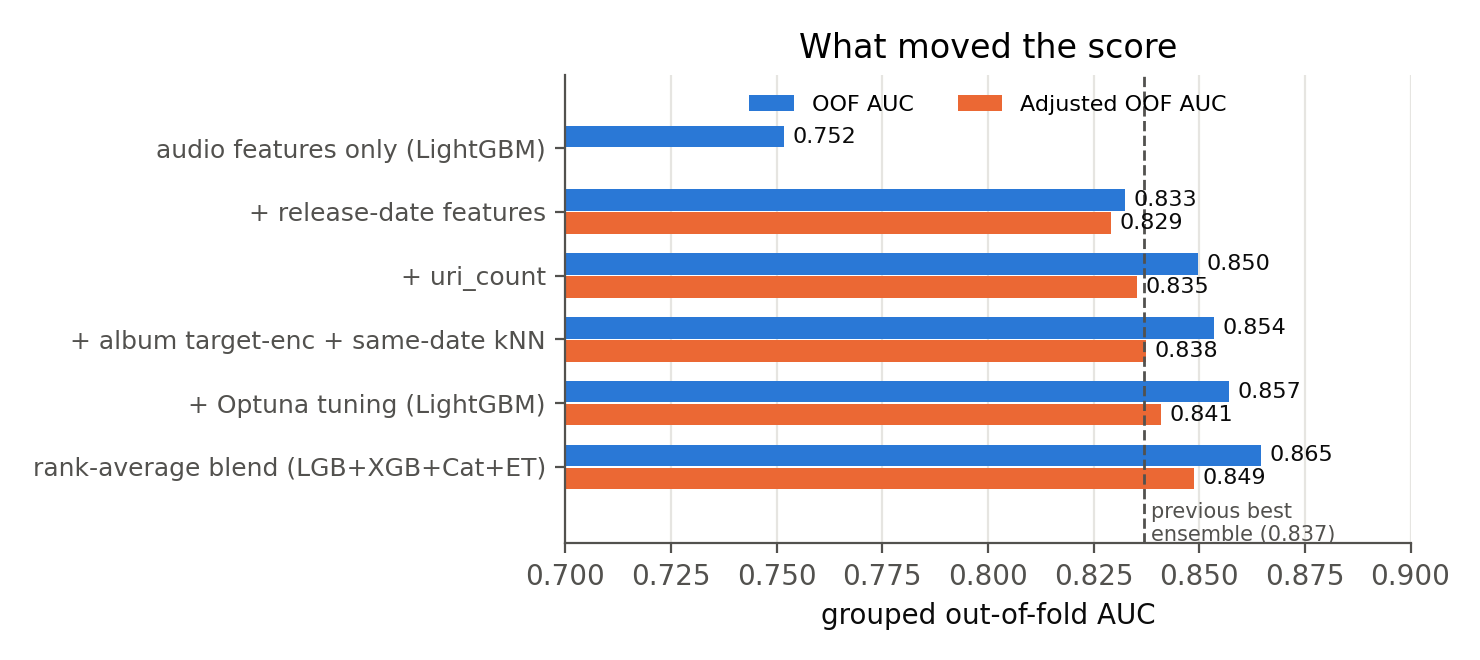
\includegraphics[width=0.64\textwidth]{../final_pipeline/figures/fig_ablation.png}
\caption{Validation gains from data analysis, feature additions, tuning, and
the final ensemble.}
\label{fig:ablation}
\end{figure}

\textit{Adjusted OOF AUC} downweights repeated tracks to match their test-set
frequency. LightGBM and XGBoost tied as the strongest individual models at
0.8435 adjusted AUC, followed by CatBoost (0.8413) and Extra Trees (0.8375).
Their different errors raised the rank-average ensemble to 0.8487
(Appendix Section~\ref{app:progression}).

\subsection{Validation and test}
We first used five-fold stratified cross-validation, then used ten folds and
five random seeds for the final comparison. Folds were grouped by URI, so all
copies of one track stayed together, while stratification kept similar class
ratios across folds. Every row received an out-of-fold prediction. Features
based on labels were calculated only from the training portion of each fold.
We averaged the fold and seed predictions for the unlabeled competition test
set.

Because repeated URIs were more common in training, adjusted OOF gave a more
realistic estimate (Appendix Section~\ref{app:validation}).

\begin{center}
\footnotesize
\setlength{\tabcolsep}{6pt}
\renewcommand{\arraystretch}{1.08}
\begin{tabularx}{0.88\textwidth}{@{}>{\raggedright\arraybackslash}X
  >{\raggedright\arraybackslash}p{0.18\textwidth}
  >{\raggedright\arraybackslash}p{0.32\textwidth}@{}}
\toprule
\textbf{Evaluation} & \textbf{AUC} & \textbf{What it showed} \\
\midrule
Grouped OOF & 0.8646 & Best local ranking estimate, but duplicates increased it. \\
Adjusted OOF & 0.8487 & More realistic estimate for the competition test set. \\
Kaggle public leaderboard & 0.87013 & Strong result on the smaller public split. \\
Kaggle private leaderboard & 0.84087 & Final score; rank 18 and top 50\%. \\
\bottomrule
\end{tabularx}
\end{center}

\newpage

\section{Conclusion [20 points]}
% 1 page maximum
\subsection{Insights}
We ranked features within each final model and averaged those ranks across
LightGBM, XGBoost, CatBoost, and Extra Trees. This avoids comparing raw
importance values that use different scales. The directions below come from
class averages and rank correlations; they describe general trends, not
causal effects.

\begin{center}
\footnotesize
\setlength{\tabcolsep}{6pt}
\renewcommand{\arraystretch}{1.05}
\begin{tabularx}{0.92\textwidth}{@{}r
  >{\raggedright\arraybackslash}p{0.37\textwidth}
  >{\raggedright\arraybackslash}X@{}}
\toprule
\textbf{Rank} & \textbf{Feature} & \textbf{Observed influence} \\
\midrule
1 & Same-date neighbor score & Higher scores favored High popularity. \\
2 & Loudness--energy interaction & Important nonlinear interaction; no single direction. \\
3 & Instrumentalness & Higher values favored Low popularity. \\
4 & Release-date position & More recent dates generally favored Low popularity. \\
5 & Log instrumentalness & Higher values favored Low popularity. \\
6 & URI count & Tracks appearing more often favored High popularity. \\
7 & Track age in days & Older tracks favored High popularity. \\
8 & Log track age & Older tracks favored High popularity. \\
9 & Release year & More recent years generally favored Low popularity. \\
10 & Loudness & Louder tracks generally favored High popularity. \\
\bottomrule
\end{tabularx}
\end{center}

Release timing and track repetition were the strongest signals. Album
similarity, instrumentalness, and loudness were also important. The largest
gains came from understanding these patterns and processing them carefully,
rather than only increasing model complexity.

We learned how logistic regression differs from several forms of boosted
decision trees and how LightGBM, XGBoost, and CatBoost control tree growth.
We also learned to use Optuna to tune depth, learning rate, tree count,
sampling, and regularization. We learned that random seeds change fold
assignments and model randomness. We repeated ten-fold training with five
seeds and averaged their predictions, which reduced variance and made the
results more stable. Averaging diverse model families improved ranking
stability further; Appendix Section~\ref{app:ensemble} gives the full
procedure.

\subsection{Challenges}
The main challenge was overfitting during both model tuning and leaderboard
selection. Our best public score was 0.87013, while the private score was
0.84087. The smaller public split was more variable, and repeatedly reacting
to it risked selecting changes that did not generalize. Grouped validation and
the adjusted OOF score gave a more realistic estimate.

Repeated URIs were distributed differently between training and test data,
which made ordinary validation optimistic. Album features based on labels
also created a leakage risk, so they required inner grouped folds. Training
many models across folds and seeds was computationally expensive. The leakage
controls are summarized in Appendix Section~\ref{app:validation}.

With more time, we would reserve an untouched URI-grouped holdout set before
tuning, set a fixed submission budget, and use nested cross-validation for the
final comparison. We would also identify the duplicate and album structure
earlier, since these data issues mattered more than testing many weak models.
\newpage

\section{Extra Credit [5 points]}

\subsection{Why use AUC, and is there a better metric?}
AUC measures whether the model ranks High-popularity tracks above
Low-popularity tracks across every possible classification threshold. This is
useful because the competition asks for probability scores and does not define
the cost of a false positive or false negative. It is also less affected by
class imbalance than accuracy. Rank averaging worked well partly because it
directly preserves the ordering that AUC evaluates.

For this competition, AUC is a reasonable primary metric. In a real
application, a different metric could be better depending on the goal.
Precision at \(k\) would be useful if a service could promote only a fixed
number of tracks. Log loss or the Brier score would be better if accurate
probabilities, rather than only ranking, were important. F1 score or accuracy
would require choosing a threshold and error costs that this project does not
provide.

\subsection{Can our methods or pipelines be parallelized?}
Yes. Models from different cross-validation folds, random seeds, and model
families are independent and can be trained at the same time. Optuna trials
can also run in parallel because each trial evaluates a separate
hyperparameter configuration. Within a model, LightGBM, XGBoost, and Extra
Trees can use multiple CPU cores, while CatBoost and XGBoost can use a GPU.

Our final run used four model families, ten folds, and five seeds, giving many
independent training jobs. Their out-of-fold and test predictions only need to
be combined after training. In practice, we would limit concurrent jobs to
avoid exhausting memory, oversubscribing CPU cores, or making several jobs
compete for one GPU.

\subsection{What additional data would be useful?}
Artist history, follower counts, genre, record label, playlist placements,
marketing exposure, and time-stamped stream or chart counts would help explain
popularity beyond audio properties. Popularity depends heavily on audience
reach and promotion, which cannot be inferred from loudness, tempo, or
danceability alone. Time-series data could also show whether a track is
steadily growing or experiencing a short-lived spike.

These fields would need a fixed collection date before the prediction target
is measured. Otherwise, later stream counts or playlist placements could
directly reveal the label and create leakage. We did not use any such external
data in this project; these are suggestions for a future dataset.

\newpage

\section{LLM Usage}
This section has an example of LLM usage reporting below. Please follow this format to report LLM usage. Indicate each usage clearly.
\begin{itemize}
  \item Name of LLM(s) Used: ChatGPT
  \item Components of Project involving LLM: Data processing.
\end{itemize}

\subsection{Data preprocessing (example)}

\subsubsection{Interaction (example)}
Only include the parts of the response that you integrated into your project. You may submit screenshots. For example, Figure \ref{fig:llm-output} illustrates the interaction with LLM for data preprocessing.
Alternatively, you can also write out the prompt and response in text.

\subsubsection{Usage/Integration of Responses (example)}

As shown in Figure~\ref{fig:data-prep-integration}, We used the response as follows, modifying the name of the encoder object and applying it to our training dataframe data, in column some\_column.

\IfFileExists{figs/llm_report_1.png}{
  \begin{figure}[htbp]
    \centering
    \includegraphics[width=0.68\textwidth]{figs/llm_report_1.png}
    \caption{Interaction with LLM for data preprocessing.}
    \label{fig:llm-output}
  \end{figure}
}{}

\IfFileExists{figs/llm_report_2.png}{
  \begin{figure}[t]
    \centering
    \includegraphics[width=0.68\textwidth]{figs/llm_report_2.png}
    \caption{Integration of LLM's output for data preprocessing.}
    \label{fig:data-prep-integration}
  \end{figure}
}{}

\clearpage
\appendix
\section{Appendix}
\setcounter{secnumdepth}{2}

\subsection{Why we chose each model}
\label{app:models}
\begin{center}
\footnotesize
\setlength{\tabcolsep}{5pt}
\renewcommand{\arraystretch}{1.08}
\begin{tabularx}{0.97\textwidth}{@{}>{\raggedright\arraybackslash}p{0.19\textwidth}
  >{\raggedright\arraybackslash}p{0.37\textwidth}
  >{\raggedright\arraybackslash}X@{}}
\toprule
\textbf{Model} & \textbf{Reason for testing} & \textbf{Final role} \\
\midrule
L2 logistic regression & Simple, interpretable baseline for measuring linear
signal. & Established a 0.7216 AUC baseline; not ensembled. \\
LightGBM & Fast gradient boosting with detailed controls for tree growth and
regularization. & Strong individual model and final ensemble member. \\
XGBoost & A second boosted-tree implementation with different split and
regularization behavior. & Strong individual model and final ensemble member. \\
CatBoost & Handles categorical features directly and uses a different
boosting procedure. & Added diversity to the final ensemble. \\
Extra Trees & Randomized, independently fitted trees produce different errors
from boosting. & Added bagging diversity to the final ensemble. \\
\bottomrule
\end{tabularx}
\end{center}

\subsubsection{Baseline preprocessing}
\begin{compactitem}
  \item Numeric audio features: filled missing values with column medians and
  standardized.
  \item Mode: kept as a binary feature.
  \item Key and time signature: one-hot encoded with unknown categories
  ignored.
  \item Logistic model: L2 penalty, balanced class weights, and \(C=0.1\).
\end{compactitem}

\subsection{Experiment progression}
\label{app:progression}
\begin{center}
\footnotesize
\setlength{\tabcolsep}{5pt}
\renewcommand{\arraystretch}{1.08}
\begin{tabularx}{0.94\textwidth}{@{}>{\raggedright\arraybackslash}X
  >{\centering\arraybackslash}p{0.16\textwidth}
  >{\centering\arraybackslash}p{0.18\textwidth}@{}}
\toprule
\textbf{Experiment} & \textbf{Grouped OOF AUC} &
\textbf{Adjusted OOF AUC} \\
\midrule
Audio-only LightGBM & 0.7517 & --- \\
Add release-date features & 0.8325 & 0.8292 \\
Add URI count & 0.8497 & 0.8353 \\
Add album target encoding and same-date KNN & 0.8536 & 0.8375 \\
Tune LightGBM with Optuna & 0.8571 & 0.8410 \\
Four-model rank-average ensemble & \textbf{0.8646} & \textbf{0.8487} \\
\bottomrule
\end{tabularx}
\end{center}

\subsubsection{Main findings}
\begin{compactitem}
  \item Release-date features produced the largest single improvement.
  \item URI count captured the strong signal from repeated tracks.
  \item Album and same-date KNN features added smaller but repeatable gains.
  \item Optuna tuning improved each tree family, while the final ensemble
  reduced model-specific ranking errors.
\end{compactitem}

\begin{figure}[H]
\centering
\captionsetup{font=footnotesize,skip=2pt}
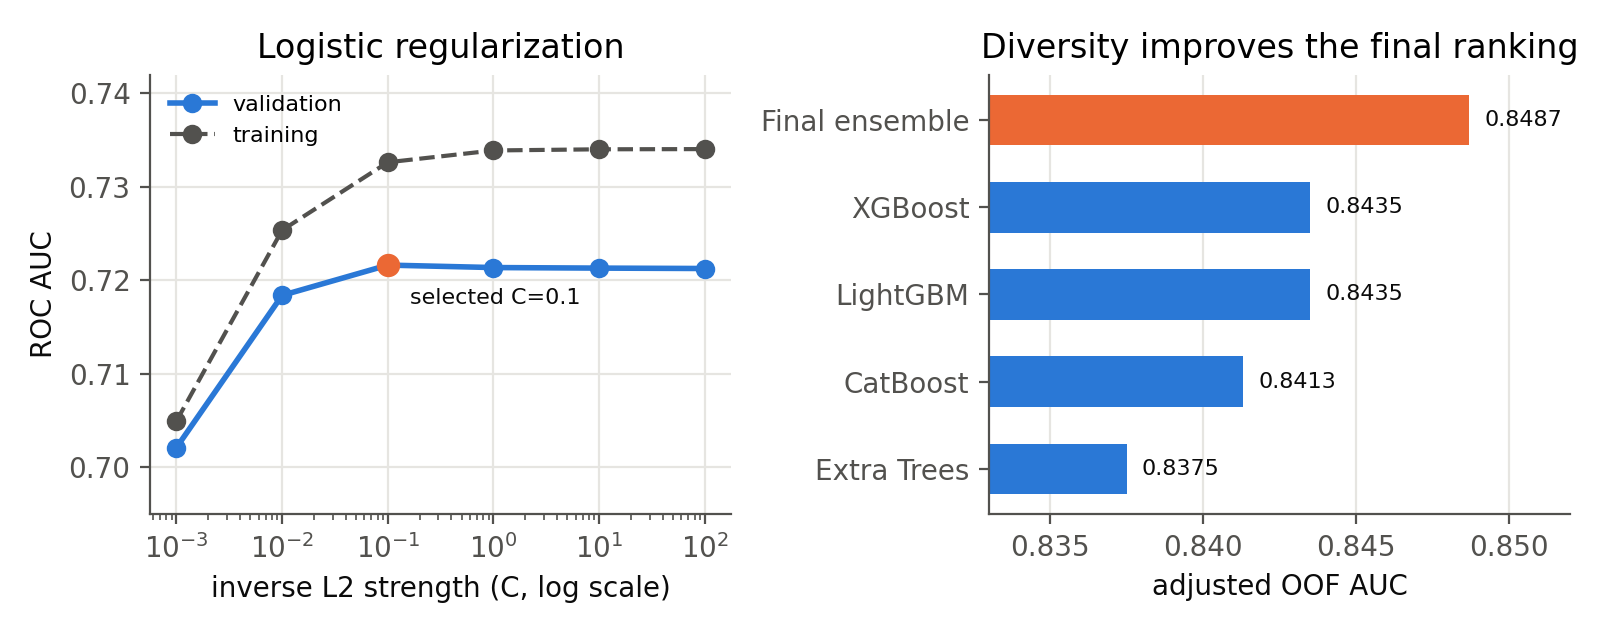
\includegraphics[width=0.82\textwidth]{../final_pipeline/figures/fig_appendix_experiments.png}
\caption{Left: logistic regression was insensitive once \(C\) reached 0.1.
Right: the rank-average ensemble outperformed every individual model under
adjusted OOF AUC.}
\label{fig:appendix-experiments}
\end{figure}

\subsection{Why we used a same-date KNN feature}
\label{app:knn}
\subsubsection{Motivation}
\begin{compactitem}
  \item Exact release dates often group tracks from the same album or release.
  \item Tracks in one release share artist, promotion, audience, and time
  period, none of which were directly provided.
  \item Audio similarity helps distinguish likely album-mates when many tracks
  share a release date.
  \item Figure~\ref{fig:release-era} shows why release timing was worth
  modeling: popularity-label rates changed substantially across release eras.
\end{compactitem}

\begin{figure}[H]
\centering
\captionsetup{font=footnotesize,skip=2pt}
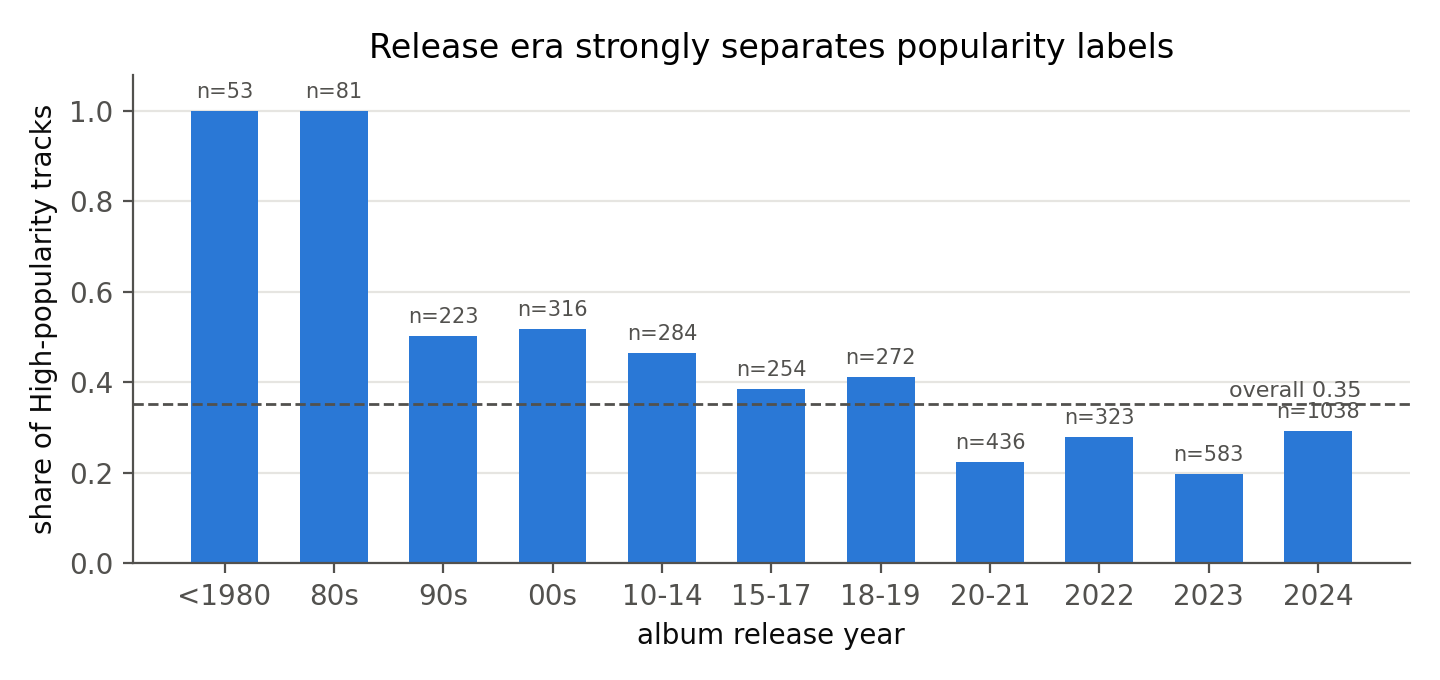
\includegraphics[width=0.58\textwidth]{../final_pipeline/figures/fig_year_rate.png}
\caption{The share of High-popularity labels varied strongly with release
era. Counts above each bar show the number of training rows.}
\label{fig:release-era}
\end{figure}

\subsubsection{Construction}
\begin{compactenum}
  \item Log-transform duration and instrumentalness, then standardize the ten
  audio features.
  \item Restrict candidate neighbors to tracks with the same exact release
  date.
  \item Select the five nearest candidates by Euclidean distance in the
  normalized audio space.
  \item Weight each neighbor by \(1/(1+d)\), where \(d\) is its distance.
  \item Average the neighbor labels with a global-mean prior of weight 2.
  \item Supply both the smoothed label mean and nearest-neighbor distance to
  the tree models.
\end{compactenum}

\subsubsection{Why it was a feature, not a KNN classifier}
KNN alone relied too heavily on local similarity and ignored broader
nonlinear patterns. Supplying the KNN score to the tree models allowed them to
combine local album evidence with release age, URI count, audio interactions,
and other features.

\subsubsection{Leakage prevention}
\begin{compactitem}
  \item Validation and test neighbors came only from the outer fold's training
  rows.
  \item Training-row scores excluded the row itself and zero-distance copies.
  \item URI grouping kept all copies of one track in the same outer fold.
\end{compactitem}

\subsubsection{Measured contribution}
\begin{center}
\footnotesize
\setlength{\tabcolsep}{7pt}
\renewcommand{\arraystretch}{1.08}
\begin{tabular}{@{}lcc@{}}
\toprule
\textbf{Feature set} & \textbf{Grouped OOF} & \textbf{Adjusted OOF} \\
\midrule
Through URI count & 0.8497 & 0.8353 \\
Add album target mean and same-date KNN & 0.8536 & 0.8375 \\
\textbf{Improvement} & \textbf{+0.0039} & \textbf{+0.0022} \\
\bottomrule
\end{tabular}
\end{center}

\subsection{Final model configurations}
\label{app:configs}
\subsubsection{Tuning process}
\begin{compactitem}
  \item Optuna searched tree size, learning rate, row sampling, feature
  sampling, and regularization.
  \item Promising settings were rerun under identical grouped folds.
  \item Selection used adjusted OOF AUC rather than training AUC or a single
  public leaderboard result.
\end{compactitem}

\begin{center}
\scriptsize
\setlength{\tabcolsep}{4pt}
\renewcommand{\arraystretch}{1.08}
\begin{tabularx}{0.98\textwidth}{@{}>{\raggedright\arraybackslash}p{0.14\textwidth}
  >{\raggedright\arraybackslash}X@{}}
\toprule
\textbf{Model} & \textbf{Final configuration} \\
\midrule
LightGBM & 1,400 trees; learning rate 0.0104; 22 leaves; depth 6;
minimum child size 11; row sample 0.555; feature sample 0.572; L1 0.0016;
L2 0.0029; extra-trees split mode. \\
XGBoost & 800 trees; learning rate 0.0090; depth 8; minimum child weight
2.46; row sample 0.644; tree feature sample 0.422; L1 0.458; L2 0.271;
\(\gamma=0.787\). \\
CatBoost & 800 iterations; learning rate 0.03; depth 6; leaf L2 5;
random strength 1; Bayesian bootstrap with temperature 0.5; 128 numeric
split borders. \\
Extra Trees & 800 trees; minimum leaf size 3; 50\% of features considered
per split. \\
\bottomrule
\end{tabularx}
\end{center}

\subsection{Additional feature construction}
\label{app:features}
\subsubsection{Release-date features}
\begin{compactitem}
  \item Year, month, day, and date precision
  \item Ordinal date, age in days, and log age
  \item Day of week, day of year, and Friday indicator
\end{compactitem}

\subsubsection{Audio transformations}
\begin{compactitem}
  \item Log transforms for duration, instrumentalness, speechiness,
  acousticness, and liveness
  \item Loudness--energy, danceability--valence, and danceability--energy
  interactions
  \item Energy minus acousticness, tempo distance from 120 BPM, and loudness
  divided by energy
\end{compactitem}

\subsubsection{Track and album features}
\begin{compactitem}
  \item URI count was calculated separately within train and test.
  \item Date-group size counted distinct tracks sharing an exact release date.
  \item Exact-date target means used prior smoothing and inner grouped folds.
\end{compactitem}

\subsection{Ensemble construction}
\label{app:ensemble}
\subsubsection{Fold and seed bagging}
\begin{compactitem}
  \item Ten stratified folds were grouped by URI.
  \item Seeds 0--4 changed fold assignment and model randomness.
  \item This produced 50 validation fits per model and reduced dependence on
  one favorable split.
  \item Fold and seed test predictions were averaged within each model.
\end{compactitem}

\subsubsection{Rank averaging}
\begin{compactitem}
  \item Each model's averaged predictions were converted to percentile ranks.
  \item The four rank vectors were averaged with equal weight.
  \item Ranking removed differences in probability scale between model
  families and matched the AUC objective.
\end{compactitem}

\subsection{Validation details}
\label{app:validation}
\subsubsection{Label-derived features}
\begin{compactitem}
  \item Date target means and KNN labels were rebuilt inside every outer fold.
  \item Training-row date means came from an additional five-fold split
  grouped by URI.
  \item No validation label was used to create its own features.
\end{compactitem}

\subsubsection{Adjusted OOF AUC}
\begin{compactitem}
  \item Duplicate URIs represented about 11\% of training rows but only 2.5\%
  of test rows.
  \item Ordinary OOF AUC therefore gave too much influence to repeated tracks.
  \item Unique rows retained weight 1; duplicate rows were downweighted until
  their total share matched the test set.
  \item The adjusted estimate, 0.8487, was closer to the private score of
  0.84087 than ordinary OOF or the public score.
  \item Final changes had to improve grouped and adjusted AUC across multiple
  seeds; the public score was only supporting evidence.
\end{compactitem}

\end{document}
